%<*driver>
\def\nameofplainTeX{plain}
\ifx\fmtname\nameofplainTeX
\input l3docstrip.tex
\keepsilent
\askforoverwritefalse
\preamble

========================================================================
 tagpax - import of tagged PDF documents

 (C) 2022-2026 Matthias Werner
 E-mail: matthias.werner@informatik.tu-chemnitz.de

 Released under the LaTeX Project Public License v1.3c or later
 See http://www.latex-project.org/lppl.txt
======================================================================== 

\endpreamble
\postamble
 This work is "maintained" (as per LPPL maintenance status) by
 Matthias Werner.
\endpostamble

\generate{
  \file{tagpax.sty}{\from{tagpax.dtx}{package}}
  \file{tagpax-tagpdf-bridge.sty}{\from{tagpax.dtx}{tagpdf-bridge}}
}
\expandafter\endbatchfile
\fi
%</driver>
%<*package>
\NeedsTeXFormat{LaTeX2e}[2024-11-01]
\ProvidesExplPackage{tagpax}
{2026/07/23}
{v0.8.5-dev}
{import of tagged PDF documents}
%</package>
%<*driver> 
\DocumentMetadata{}
\documentclass[
load-preamble+
]{osgdoc}

%\OnlyDescription

\usepackage[
  languages={de,en},
  map={de=german,en=english},
  targetlang={job=2},
  load babel
]{langselect}
\usepackage{microtype}
\usepackage{booktabs}
\usepackage{enumitem}
\usepackage{tikz}
\usetikzlibrary{arrows.meta,backgrounds,fit,positioning}

\newpackagename{\pdfpagespkg}{pdfpages}
\newpackagename{\tagpdfpkg}{tagpdf}
\newpackagename{\luatexname}{LuaTeX}
\newpackagename{\tagpaxpkg}{tagpax}

\newcommand{\luasig}[1]{\code{\detokenize{#1}}}
\newenvironment{luafunctions}
  {\begin{cnltxlist}}
  {\end{cnltxlist}}
\NewDocumentCommand\DescribeLuaFunction{m}
  {\item\luasig{#1}\hfill\newline}

\makeindex
\setcnltx{
  package  = tagpax,
  version  = \UseVersionOf{tagpax.sty},
  date     = \UseDateOf{tagpax.sty},  
  title       = {\ldeen{Das \pkg{tagpax}-Paket}{The \pkg{tagpax} package}},
  info        = {\ldeen{Semantischer Import getaggter PDF-Dokumente}{Semantic import of tagged PDF documents}},
  authors     = {Matthias Werner},
  abstract    = {\ldeen*{
    @1 ist ein experimentelles Lua\LaTeX-Paket zum Zusammenstellen vollständig
    getaggter PDF-Dokumente. Es übernimmt Seiten, logische Dokumentstruktur und
    Navigation in ein neues Masterdokument.

    Das Paket gehört zum \pkg*{osglecture}-Bundle, kann aber auch eigenständig
    genutzt werden. 
  }{
    @1 is an experimental Lua\LaTeX\ package for assembling fully tagged
    pdf documents. It imports pages, logical document structure and navigation
    into a new master document. 

    The package is part of the \pkg*{osglecture} bundle, but can also be used independently.
  }{\tagpaxpkg}
  },
  build-title
}

\begin{document}

\section{\ldeen{Ziel und Anwendungsbereich}{Purpose and scope}}

\ldeen*{
  Es gibt häufig den Fall, dass fertige PDF-Dokumente in andere eingebaut werden, beispielsweise bei Proceedings 
  und Sammelbänden. Dafür hat sich \name{Andreas Matthias}' umfangreiches Paket \needpackage{pdfpages} bewährt.
  Um aus den eingebundenen Dokumenten PDF-Annotationen zu übernehmen, beispielsweise zur Erstellung von gemeinsamen
  Inhaltsverzeichnissen, kann zusätzlich \name{Ulrike Fischer}s \needpackage{newpax} oder dessen auf Java basierendes Vorgängerprojekt \needpackage{pax} von \name{Heiko Oberdiek} genutzt werden.

  Jedoch gibt es aus der Perspektive der Barrierefreiheit ein Problem: Auch wenn die eingebundenen Dokumente
  (über \cs{MetaDocumentdata}) korrekt getaggt sind, gehen diese Informationen beim Einbinden verloren.
  Dies war der Anstoß für die Schaffung von \tagpaxpkg, das die Möglichkeit gibt, Tagging-Informationen in
  das Gesamtdokument zu übernehmen.
}{
  It is often the case that finished PDF documents are embedded into others, for example in proceedings 
  and anthologies. \name{Andreas Matthias}’s comprehensive package \needpackage{pdfpages} has proven useful for this purpose.
  To extract PDF annotations from the embedded documents-—for example, to create combined
  tables of contents-—you can also use \name{Ulrike Fischer}’s \needpackage{newpax} or its Java-based predecessor project, \needpackage{pax}, by \name{Heiko Oberdiek}.

  However, there is a problem from an accessibility perspective: Even if the embedded documents
  are correctly tagged (via \cs{MetaDocumentdata}), this information is lost during embedding.
  This was the impetus for the creation of \tagpaxpkg, which allows tagging information to be
  incorporated into the overall document.
}
\medskip

\begin{infobox}{\ldeen{Achtung}{Note}}
    \ldeen*{
      Dieses Paket ist \textbf{kein} Ersatz für die oben genannten Pakete @1 und @2.
      Es ist (zumindest derzeit) nur auf den Anwendungsfall der Inkludierung von vollständigen,
      korrekt getaggten PDF-Dokumenten in der Originalreihenfolge der Seiten ausgelegt.
      Die vielfältigen Möglichkeiten zu weiteren Manipulation sind in \tagpaxpkg{} nicht möglich.
      }{
      This package is \textbf{not} a substitute for the pakets @1 and @2 mentioned above.
      It is (at least for now) designed only for the specific use case of including complete,
      correctly tagged PDF documents in their original page order.
      The various options for further manipulation are not available in \tagpaxpkg.
    }{\pkg{pdfpages}}{\pkg{pax}/\pkg{newpax}}
\end{infobox}
\medskip


\ldeen*{Beim Einbinden eines Subdokuments wird seine äußere
  @1-Struktur entfernt; ihre Kinder werden im Master unter
  einem neuen @2 eingehängt. Vorhandene MCIDs bleiben dabei erhalten.
}{When a subdocument is embedded, its outer
  @1 structure is removed; its children are attached to the master under
  a new @2. Existing MCIDs are preserved in the process.
}{\code{Document}}{\code{Part}}

\section{\ldeen{Nutzung}{Usage}}
\subsection{\ldeen{Schnellstart}{Quick start}}
\ldeen*{
  Aktivieren Sie PDF-Management und automatisches Tagging vor der Dokumentklasse
  mit @1 sowohl in den Subdokumenten, als auch im Masterdokument.
}{
  Enable PDF management and automatic tagging before the document class
   in both the subdocuments and the master document using @1. 
}{\cs{DocumentMetadata}\Marg{tagging=on}}

\begin{Verbatim}
\DocumentMetadata{tagging=on}
\documentclass{book}
\usepackage{tagpax}
\end{Verbatim}

\ldeen*{
  Um ein getaggtes Dokument einzubinden, extrahieren Sie zunächst die semantische Zwischenrepräsentation mit @1 und importieren Sie anschließend das vollständige Dokument mit @2.
}{
   To embed a tagged document, first extract the semantic intermediate representation using @1, and then import the complete document using @2.
}{\cs{tagpaxextract}}{\cs{tagpaxinclude}}

\begin{Verbatim}
\tagpaxextract[paper.tagpax]{paper.pdf}
\tagpaxinclude[ir=paper.tagpax]{paper.pdf}
\end{Verbatim}

\ldeen*{
  Der Importer erzeugt pro Quellseite ein frisches Form-XObject, setzt
  @1 vor dem Schreiben des Forms und rekonstruiert die Seitenstream-MCRs unter
  einem neuen @2. Explizite verschachtelte @3-Streams sind im gegenwärtigen MVP
  noch nicht importierbar.
}{
  The importer creates a fresh Form XObject for every source page, sets
  @1 before the Form is written and reconstructs page-stream MCRs below a new
  @2. Explicit nested @3 streams are not yet importable by the current MVP.
}{\code{/StructParents}}{\code{Part}}{\code{/Stm}}

\subsection{\ldeen*{Optionale @1-Kompatibilität}{Optional @1 compatibility}{\pdfpagespkg}}

\ldeen*{
  Für eine schnelle Migration kann die Paketoption @1 die vertraute @2-Syntax bereitstellen.
  Unterstützt werden nur der lineare Vollimport mit @3 und @4. Die Option lädt
  @5 nicht; die eigentliche Form-Erzeugung übernimmt der native Importer.
}{
  For a quick migration, the package option @1 can provide the familiar @2 syntax. It supports
  only linear full-document import with @3 and @4. The option does not load @5;
  actual Form creation remains the responsibility of the native importer.
}{\keyis*-{pdfpages}{true}}{\cs{includepdf}}{\keyis{pages}{-}}{\option{pagecommand}}{\pkg{pdfpages}}

\begin{Verbatim}
\usepackage[pdfpages]{tagpax}
\includepdf[
  pages=-,
  pagecommand={\thispagestyle{empty}}
]{paper.pdf}
\end{Verbatim}

\begin{infobox}{\ldeen{Hinweis}{Hint}}
\ldeen*{
  Aktivieren Sie diese Option nicht zusammen mit dem echten @1-Paket, das könnte zu 
  Problemen führen.
  Wenn @2 @1 erkennt, deaktiviert es seinen Kompatibilitätsbefehl und gibt
  eine Warnung aus. Verwenden Sie in einem solchen Dokument für semantische Importe
  ausschließlich @3.
}{
  Do not enable this option together with the real @1 package; doing so could 
  cause problems.
  If @2 detects @1, it disables its compatibility directive and issues
  a warning. In such a document, use only @3
  for semantic imports.
}{\pkg{pdfpages}}{\pkg{tagpax}}{\cs{tagpaxinclude}}


\ldeen*{
  Optionen wie @1, @2, @3, beliebige Seitenauswahlen und wiederholte Seiten
  werden abgelehnt, weil (zumindest derzeit) vollständige lineare
  Beiträge voraussetzt werden.
}{
  Options such as @1, @2, @3, arbitrary page selections, and repeated pages
  are rejected because (at least for now) complete linear
  posts are required.
}{\option{nup}}{\option{booklet}}{\option{signature}}
\end{infobox}

\subsection{\ldeen{Konfiguration}{Configuration}}
\label{sec:config}
\ldeen{Um die Stukturen korrekt in das aufnehmende Dokument einzupassen, kann das Tagging konfiguriert werden.}{
  To ensure that the structures are correctly integrated into the target document, the tagging can be configured.}

\begin{Verbatim}
\tagpaxsetup{
  heading-map = {H2=chapter,H3=section,H4=subsection},
  toc-depth = H4,
  bookmark-depth = H5
}
\end{Verbatim}

\ldeen*{Die Option
  Der Schlüssel @1 ordnet PDF-Überschriftenrollen den Ebenen des LaTeX-Inhaltsverzeichnisses
  zu. @2 und @3 legen die maximale Tiefe für sichtbares Inhaltsverzeichnis und
  PDF-Lesezeichen getrennt fest. Die Überschriftenrollen im importierten
  Strukturbaum werden nicht verändert.
}{
  The key @1 maps PDF heading roles to LaTeX table-of-contents levels. @2 and @3 set
  the maximum depth for the visible table of contents and PDF bookmarks
  independently. Heading roles in the imported structure tree are not changed.
}{\option{heading-map}}{\option{toc-depth}}{\option{bookmark-depth}}

\subsection{\ldeen{Befehlsübersicht}{Command Overview}}
\ldeen*{Insgesamt stellt das Paket @1 die folgende Macros zur Verfügung}{Overall, the @1 package provides the following macros}{\tagpaxpkg}:
\begin{commands}
  \command{tagpaxextract}[\oarg{\ldeen{Ausgabedatei}{output file}}\marg{\ldeen{PDF-Datei}{pdf file}}]
  \ldeen*{
    Extrahiert die kanonische Zwischenrepräsentation aus @1. Ohne explizite
    @2 wird der Dateiname aus der PDF-Datei abgeleitet.
  }{
    Extracts the canonical intermediate representation from @1. If @2 is not
    given explicitly, the filename is derived from the PDF file.
  }{\meta{PDF-Datei}}{\meta{Ausgabedatei}}
%
  \command{tagpaxinclude}[\oarg{ir=\ldeen{metadata file}{Metadaten-Datei}}\marg{\ldeen{PDF-Datei}{pdf file}}]
  \ldeen*{
    Importiert PDF-Datei mit dem nativen linearen Importer. Mit @1 kann eine bereits
    erzeugte Zwischenrepräsentation angegeben werden.
  }{
    Imports \meta{pdf file} with the native linear importer. An existing intermediate
    representation can be selected with @1.
  }{\option{ir}}
%
  \command{tagpaxlastprefix}
  \ldeen*{
    Expandierbar. Liefert den intern vergebenen Präfix des zuletzt
    ausgeführten @1-Aufrufs -- z.\,B. um ihn extern zu protokollieren und in
    einem späteren Lauf wiederzuverwenden.
  }{
    Expandable. Returns the internally assigned prefix of the most recently
    executed @1 call -- e.g. to log it externally and reuse it in a later
    run.
  }{\cs{tagpaxinclude}}
%
  \command{includepdf}[\oarg{\ldeen{Optionen}{options}\marg{\ldeen{PDF-File}{pdf file}}}]
  \ldeen*{Existiert nur bei gesetzter Paketoption @1. Importiert direkt das angegeben File.}{Exists only when the @1 package option is set. It directly imports the specified file.}{\option{pdfpages}}
%
\begin{quotation}
  \begin{options}
    \keyval*{pages}{\ldeen{Seitenbereich}{page range}}\Default{-}
    \ldeen{Seitenauswahl, kein anderer Wert möglich.}{Page selection; no other value is possible.}
    \keyval*{pagecommand}{\ldeen{Ausdruck}{expression}}\Default{\code{\{\cs{thispagestyle}\Marg{empty}\}}}
    \ldeen{Deklariert \LaTeX-Befehle, die für jede Seite ausgeführt werden.}{Declares \LaTeX\ commands, which are executed on each sheet of paper.}
  \end{options}
  \ldeen*{Andere @1-Optionen sind nicht gültig.}{Other @1 options are not valid.}{\pdfpagespkg}
\end{quotation}

  \command{tagpaxsetup}[\marg{\ldeen{Optionen}{options}}]
  \ldeen{Legt die globalen Import- und Navigationsoptionen fest.}
         {Sets global import and navigation options.}

  \begin{quotation}
    \begin{options}
      \keyval*{heading-map}{\ldeen{Zuordnung}{mappings}}\default{}
      \keyval*{toc-depth}{\ldeen{Headerlevel}{header level}}\default{}    
      \keyval*{bookmark-depth}{\ldeen{Headerlevel}{header level}}\default{}
      \ldeen*{Siehe Abschnitt~@1}{See Section~@1}{\ref{sec:config}}
  \end{options}
  \end{quotation}
  
\end{commands}

\section{Developer manual}

\subsection{\ldeen{Entwicklungsstand}{Development status}}

\ldeen*{
  Der aktuelle Stand ist für Experimente mit selbst erzeugten, korrekt
  getaggten Dokumenten geeignet, aber noch nicht sehr robust.
  Ein semantischer Roundtrip wird durch @1
  geprüft. Seitenstream-MCRs, Link-Annotationen und lokale Ziele werden
  rekonstruiert. Explizite verschachtelte Form-XObjects bleiben außerhalb des
  unterstützten Importprofils.
}{
  The current state is suitable for experiments with self-generated, correctly
  tagged documents. A semantic roundtrip is tested by @1. Page-stream MCRs,
  link annotations and local destinations are reconstructed. Explicit nested
  Form XObjects remain outside the supported import profile.
}{\code{l3build check -c roundtrip}}

\subsection{\ldeen{Architektur}{Architecture}}
%\begin{center}
\resizebox{\linewidth}{!}{%
\fbox{
  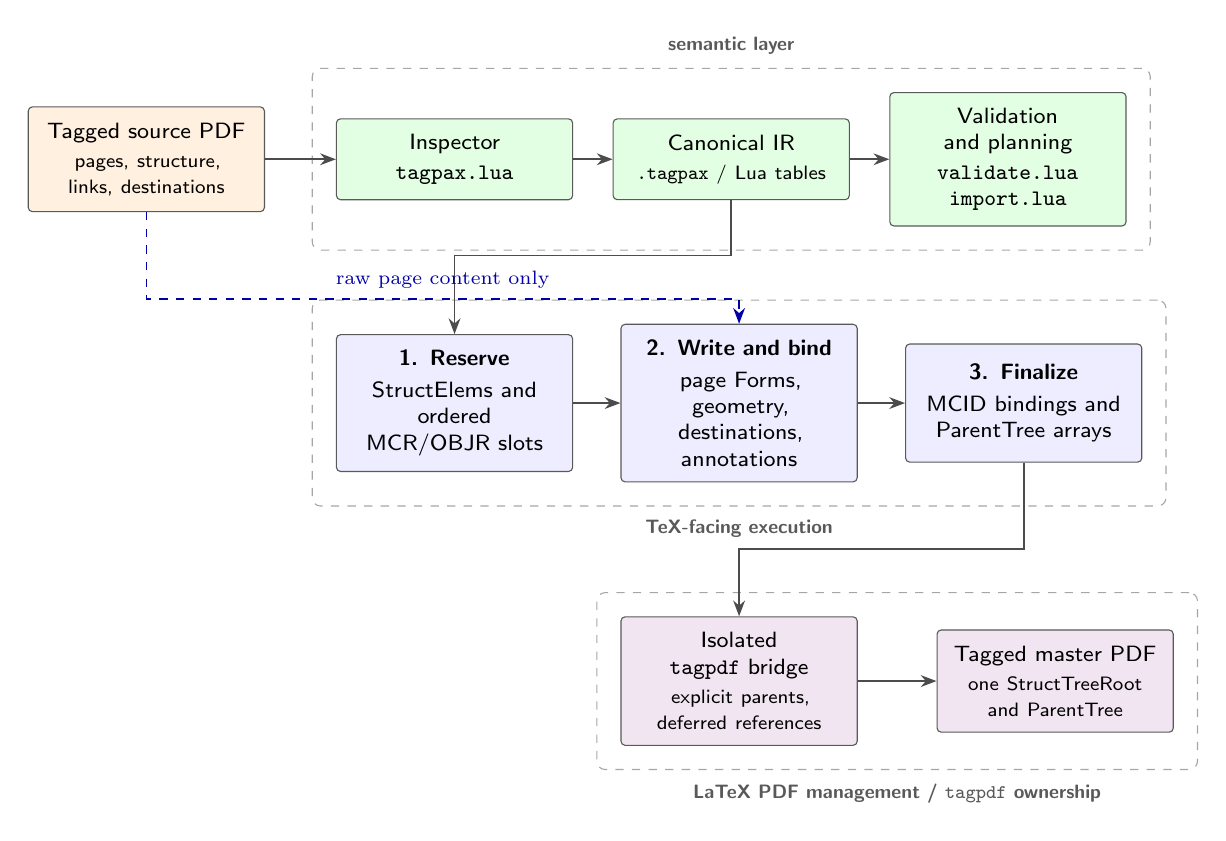
\begin{tikzpicture}[
  font=\sffamily\footnotesize,
  >={Stealth[length=2mm]},
  flow/.style={->, semithick, draw=black!70},
  late/.style={->, semithick, dashed, draw=blue!65!black},
  box/.style={
    draw=black!65,
    rounded corners=1.5pt,
    align=center,
    text width=26mm,
    inner sep=2mm,
    fill=white
  },
  source/.style={box, fill=orange!12},
  semantic/.style={box, fill=green!11},
  execution/.style={box, fill=blue!9},
  owner/.style={box, fill=violet!10},
  phase/.style={box, minimum height=15mm, fill=blue!7},
  boundary/.style={
    draw=black!35,
    rounded corners=3pt,
    dashed,
    inner sep=3mm
  },
  zonelabel/.style={font=\sffamily\scriptsize\bfseries, text=black!65, label distance=0.5mm}
]

% The top row is the stable semantic pipeline.  PDF object identities stop at
% the inspector; all following components communicate through canonical IR.
\node[source] (pdf) {Tagged source PDF\\[1pt]
  \scriptsize pages, structure, links, destinations};
\node[semantic, right=9mm of pdf] (inspect) {Inspector\\[1pt]
  \texttt{tagpax.lua}};
\node[semantic, right=5mm of inspect] (ir) {Canonical IR\\[1pt]
  \scriptsize\texttt{.tagpax} / Lua tables};
\node[semantic, right=5mm of ir] (validate) {Validation and planning\\[1pt]
  \texttt{validate.lua}\\ \texttt{import.lua}};

\draw[flow] (pdf) -- (inspect);
\draw[flow] (inspect) -- (ir);
\draw[flow] (ir) -- (validate);

% Object references for Forms and annotations are allocated late.  The three
% boxes make that temporal constraint visible without implying three IRs.
\node[phase, below=17mm of inspect] (reserve) {
  \textbf{1. Reserve}\\[2pt]
  StructElems and\\ordered MCR/OBJR slots};
\node[phase, right=6mm of reserve] (write) {
  \textbf{2. Write and bind}\\[2pt]
  page Forms, geometry,\\destinations, annotations};
\node[phase, right=6mm of write] (finalize) {
  \textbf{3. Finalize}\\[2pt]
  MCID bindings and\\ParentTree arrays};

% All inter-row connectors bend inside the empty gap between rows: they drop
% to an intermediate coordinate first and only then turn, so the corner never
% grazes a neighbouring box.
\draw[flow] (ir.south) -- ++(0,-7mm) -| (reserve.north);
\draw[flow] (reserve) -- (write);
\draw[flow] (write) -- (finalize);

% The page writer deliberately reopens the source only for page content and
% final geometry; semantic PDF objects are never rediscovered on this path.
\draw[late] (pdf.south) -- ++(0,-11mm) -| (write.north)
  node[pos=0.25, above, font=\scriptsize, text=blue!65!black] {raw page content only};

\node[owner, below=17mm of write] (bridge) {Isolated \texttt{tagpdf} bridge\\[1pt]
  \scriptsize explicit parents, deferred references};
\node[owner, right=10mm of bridge] (master) {Tagged master PDF\\[1pt]
  \scriptsize one StructTreeRoot and ParentTree};

\draw[flow] (finalize.south) -- ++(0,-11mm) -| (bridge.north);
\draw[flow] (bridge) -- (master);

% Dashed frames denote ownership boundaries rather than additional runtime
% components.  In particular, tagpdf remains the sole owner of global trees.
\begin{scope}[on background layer]
  \node[boundary, fit=(inspect)(ir)(validate),
    label={[zonelabel]above:semantic layer}] {};
  \node[boundary, fit=(reserve)(write)(finalize),
    label={[zonelabel]below:TeX-facing execution}] {};
  \node[boundary, fit=(bridge)(master),
    label={[zonelabel]below:LaTeX PDF management / \texttt{tagpdf} ownership}] {};
\end{scope}

\end{tikzpicture}
}%
}
%\end{center}

\MaybeStop{
     \begin{infobox}{}
      \ldeen*{Wenn Sie die vollständige Entwicklerdokumentation sehen wollen, übersetzen Sie @1 mit auskommentierten @2.}{
      If you also want to view the complete developer documentation, translate @1 with @2 commented out.}{\code{tagpax.dtx}}{\cs*{OnlyDescription}}
    \end{infobox}
}
Source semantics are read once by the inspector and
then passed through a canonical IR. The page writer reopens the PDF only for
page content and geometry; it does not rediscover structure or navigation.

\begin{center}
  \begin{tabular}{@{}lll@{}}
  \toprule
  Layer & Input & Responsibility \\
  \midrule
  Inspector & PDF object graph & Normalise structure, streams, destinations and annotations \\
  Canonical IR & Plain Lua tables & Stable semantic document graph \\
  Transformations & Canonical IR & Unwrap \code{Document}, create contribution \code{Part}, navigation \\
  Import plan & Transformed IR + bindings & Resolve source streams to target Forms \\
  Backend plan & Import plan & Order PDF-writing operations \\
  Backend & Backend plan & Emit Forms, StructElems, MCRs, OBJRs and ParentTree entries \\
  \bottomrule
  \end{tabular}
\end{center}

The architectural rules are:
\begin{itemize}
  \item semantic processing \emph{after} inspection use the canonical IR;
  \item PDF object numbers are not semantic identifiers;
  \item MCIDs are retained and remain local to their content stream;
  \item transformations are separated from PDF-writing operations;
  \item the central \LaTeX tagging backend remains the sole owner of the ParentTree.
\end{itemize}

\subsection{Lua API}

The Lua modules form a supported developer interface. Functions documented in
this section operate on plain Lua tables and do not require TeX unless stated
otherwise. Callers should treat undocumented fields as private.

\subsubsection{Inspector: \code{tagpax-inspect}}
\begin{luafunctions}
  \DescribeLuaFunction{inspect.from_pdf(filename, output?)}
    Reads a tagged PDF with LuaTeX's \code{pdfe} library, normalises it and
    returns canonical IR. If \code{output} is supplied, the canonical
    serialisation is written as well.
  \DescribeLuaFunction{inspect.from_file(filename)}
    Reads a serialised \code{.tagpax} file.
  \DescribeLuaFunction{inspect.summary(ir)}
    Returns stable summary values for diagnostics and tests.
\end{luafunctions}

\subsubsection{IR module: \code{tagpax-ir}}
\begin{luafunctions}
  \DescribeLuaFunction{ir.new()} Creates an empty canonical IR value.
  \DescribeLuaFunction{ir.read(filename)} Parses canonical line-oriented serialisation.
  \DescribeLuaFunction{ir.count_nodes(ir)} Returns the number of structure nodes.
\end{luafunctions}

\subsubsection{Validation: \code{tagpax-validate}}
\begin{luafunctions}
  \DescribeLuaFunction{validate.validate(ir)}
    Checks referential integrity, stream bindings, root nodes, child order and
    heading references. On failure, \code{errors} is an ordered list.
\end{luafunctions}

\subsubsection{Import planning: \code{tagpax-import}}
\begin{luafunctions}
  \DescribeLuaFunction{import.plan(ir, bindings, options?)}
    Converts semantic IR into a backend-independent import plan. Page streams
    use \code{bindings.pages[page]}; explicit streams use
    \code{bindings.streams[id]}.
  \DescribeLuaFunction{import.assert_resolved(plan)}
    Reports unresolved stream bindings. Explicit \code{/Stm} bindings are never
    redirected silently to a page Form.
\end{luafunctions}

\subsubsection{LuaTeX importer: \code{tagpax-luatex}}
\begin{luafunctions}
  \DescribeLuaFunction{luatex.write_page(filename, page, structparents, stream_id, max_width?, max_height?)}
    Writes one source page as a fresh Form XObject, adds
    \code{/StructParents}, and reports its target object reference.
  \DescribeLuaFunction{luatex.page_geometry(filename, page, max_width?, max_height?)}
    Returns the shared crop, scale and rotation transformation used for the
    page Form, destination coordinates and annotation rectangles.
\end{luafunctions}

\subsubsection{Native importer: \code{tagpax-native}}
\begin{luafunctions}
  \DescribeLuaFunction{native.emit_page_imports(pdf, irfile, prefix)}
    Emits one controlled page import operation per source page. This function
    is TeX-facing and requires LuaTeX. \meta{prefix} namespaces the
    page-stream ids so multiple imports into one master document do not
    collide.
\end{luafunctions}

\subsubsection{Backend prototype: \code{tagpax-backend}}
\begin{luafunctions}
  \DescribeLuaFunction{backend.emit_reservations(filename, prefix)}
    Reserves explicit-parent StructElems and source-ordered MCR/OBJR kid slots
    before page objects exist. \meta{prefix} namespaces MCR stream ids so
    multiple imports into one master document do not collide.
  \DescribeLuaFunction{backend.emit_bindings(filename, prefix)}
    Registers the MCID bindings and commits external ParentTree arrays after
    pages and annotations have supplied their target object references.
    \meta{prefix} must match the value passed to
    \luasig{backend.emit_reservations}.
\end{luafunctions}

\subsection{Canonical intermediate representation}

The IR is the normative semantic API. A \code{.tagpax} file is its canonical
transport serialisation. IR version 1 contains source metadata, streams,
structure nodes, ordered child relations, roots, headings, destinations and
supported link annotations.

\begin{center}
\begin{tabular}{@{}llp{.52\linewidth}@{}}
\toprule
Record & Required fields & Meaning \\
\midrule
\code{source}  & \code{file}, \code{pages} & source-document identity \\
\code{stream}  & \code{id}, \code{kind} & page or explicit object stream \\
\code{node}    & \code{id}, \code{role} & structure element \\
\code{kid}     & \code{parent}, \code{index}, \code{kind} & ordered child relation \\
\code{heading} & \code{node}, \code{role}, \code{page}, \code{text} & navigation data \\
\code{destination} & \code{id}, \code{page}, \code{view} & named target and view parameters \\
\code{annotation} & \code{id}, \code{page}, \code{action}, \code{rect} & link geometry and action data \\
\code{root}    & \code{index}, \code{node} & root ordering \\
\bottomrule
\end{tabular}
\end{center}

\subsection{Backend}

The backend first reserves all structure elements and source-ordered kid slots.
It then writes Form XObjects and annotation overlays, binding their late PDF
object references into the reserved slots. Finally it commits the MCR and
annotation mappings to the central ParentTree. This three-phase order is
necessary because LuaTeX allocates Form and annotation objects during page
construction, but appending children only at that time would lose the source
\code{/K} order. Imported annotations receive \code{/StructParent} and
\code{/OBJR} entries owned by their original imported \code{Link} element;
tagpdf's automatic replacement-Link mechanism is suppressed for these overlays.
The bridge must not mutate the global \tagpdfpkg{} structure stack.

\subsection{Implementation}


\subsubsection{\code{tagpax.sty}}
\AutoDocInput{tagpax.dtx}{package}

\subsubsection{\code{tagpdf-bridge}}
\AutoDocInput{tagpax.dtx}{tagpdf-bridge}

\NewDocumentCommand{\tpdocluafile}{m}{
  \subsubsection{\code{#1}}
  \AutoDocInput[lua]{#1}{pkg}
}

\tpdocluafile{tagpax.lua}

\end{document}
%</driver>
% \fi
%
%<*package>
\RequirePackage{tagpax-tagpdf-bridge}
\ExplSyntaxOn
\bool_new:N \g__tagpax_pdfpages_compat_bool
\keys_define:nn {tagpax/package}
  {
    pdfpages .bool_gset:N = \g__tagpax_pdfpages_compat_bool,
    pdfpages .default:n = true,
  }
\ProcessKeyOptions[tagpax/package]
\msg_new:nnn {tagpax}{luatex-required}{tagpax~currently~requires~LuaLaTeX.}
\msg_new:nnn {tagpax}{metadata-required}{Activate~PDF~management/tagging~with~\string\DocumentMetadata{tagging=on}.}
\msg_new:nnn {tagpax}{backend-missing}{External-MCR~backend~not~installed;~navigation~is~generated,~structure~attachment~is~not~yet~written.}
\sys_if_engine_luatex:F {\msg_fatal:nn{tagpax}{luatex-required}}
\pdfmanagement_if_active:F {\msg_warning:nn{tagpax}{metadata-required}}
\seq_new:N \l__tagpax_headings_seq
\tl_new:N \l__tagpax_toc_depth_tl
\tl_new:N \l__tagpax_bookmark_depth_tl
\int_new:N \l__tagpax_toc_depth_int
\int_new:N \l__tagpax_bookmark_depth_int
\tl_new:N \l__tagpax_ir_tl
\tl_new:N \l__tagpax_file_tl
\tl_new:N \l__tagpax_pagecommand_tl
\tl_new:N \l__tagpax_import_id_tl
\tl_new:N \l__tagpax_import_stream_key_tl
\int_new:N \g__tagpax_import_int
\tl_new:N \g__tagpax_last_prefix_tl
\prop_new:N \g__tagpax_heading_map_prop
\prop_gput_from_keyval:Nn \g__tagpax_heading_map_prop {H2=chapter,H3=section,H4=subsection,H5=subsubsection,H6=paragraph}
\keys_define:nn {tagpax/setup}{
  toc-depth .code:n={
    \tl_set:Nn\l__tagpax_toc_depth_tl{#1}
    \int_set:Nn\l__tagpax_toc_depth_int{\tl_tail:n{#1}}
  },
  bookmark-depth .code:n={
    \tl_set:Nn\l__tagpax_bookmark_depth_tl{#1}
    \int_set:Nn\l__tagpax_bookmark_depth_int{\tl_tail:n{#1}}
  },
  heading-map .code:n=\prop_gput_from_keyval:Nn \g__tagpax_heading_map_prop {#1},
}
\keys_set:nn {tagpax/setup}{toc-depth=H4,bookmark-depth=H5}
\NewDocumentCommand\tagpaxsetup{m}{\keys_set:nn{tagpax/setup}{#1}}
\cs_new_protected:Npn \tagpax_heading_record:nnnn #1#2#3#4 {\seq_put_right:Nn\l__tagpax_headings_seq{{#1}{#2}{#3}{#4}}}
\cs_new:Npn \__tagpax_heading_num:n #1 {\tl_tail:n{#1}}
\cs_new_protected:Npn \__tagpax_build_addtotoc:N #1 {
  \tl_clear:N #1
  \seq_map_inline:Nn \l__tagpax_headings_seq {
    \__tagpax_build_addtotoc_aux:nnnnN ##1 #1
  }
}
\cs_new_protected:Npn \__tagpax_build_addtotoc_aux:nnnnN #1#2#3#4#5 {
  \int_compare:nNnT
    {\__tagpax_heading_num:n{#1}}
    <
    {\l__tagpax_toc_depth_int+1} {
    \prop_get:NnNT \g__tagpax_heading_map_prop {#1}\l_tmpa_tl {
      \tl_if_empty:NF #5 {\tl_put_right:Nn #5 {,}}
      \tl_put_right:Ne #5 {#2,\l_tmpa_tl,{\exp_not:n{#4}},tagpax.#3}
    }
  }
}
\keys_define:nn {tagpax/include}{
  ir .tl_set:N=\l__tagpax_ir_tl,
  toc-depth .code:n={
    \tl_set:Nn\l__tagpax_toc_depth_tl{#1}
    \int_set:Nn\l__tagpax_toc_depth_int{\tl_tail:n{#1}}
  },
  bookmark-depth .code:n={
    \tl_set:Nn\l__tagpax_bookmark_depth_tl{#1}
    \int_set:Nn\l__tagpax_bookmark_depth_int{\tl_tail:n{#1}}
  },
  pagecommand .tl_set:N=\l__tagpax_pagecommand_tl,
}
\msg_new:nnn {tagpax}{deprecated-command}
  {Command~\token_to_str:N #1~is~deprecated;~use~\token_to_str:N #2~instead.}
\NewDocumentCommand\tagpaxextract{O{}m}{
  \directlua{
    require('tagpax').extract_command(
      "\luaescapestring{#2}", "\luaescapestring{#1}")
  }
}
\NewDocumentCommand\TagPaxExtract{O{}m}{
  \msg_warning:nnnn {tagpax}{deprecated-command}
    {\TagPaxExtract}{\tagpaxextract}
  \tagpaxextract[#1]{#2}
}
\NewDocumentCommand\tagpaxinclude{O{}m}{
  \group_begin:
  \int_gincr:N \g__tagpax_import_int
  \tl_set:Ne \l__tagpax_import_id_tl {\int_use:N\g__tagpax_import_int}
  \tl_gset:Ne \g__tagpax_last_prefix_tl {\l__tagpax_import_id_tl}
  \tl_set:Nn \l__tagpax_file_tl {#2}
  \tl_set:Nn \l__tagpax_ir_tl {#2}
  \regex_replace_once:nnN { \.pdf\Z } {.tagpax} \l__tagpax_ir_tl
  \tl_clear:N \l__tagpax_pagecommand_tl
  \keys_set:nn {tagpax/include}{#1}
  \directlua{require('tagpax-backend').emit_reservations(
    [[\luaescapestring{\l__tagpax_ir_tl}]],
    [[\luaescapestring{\l__tagpax_import_id_tl}]])}
  \directlua{require('tagpax-native').emit_page_imports(
    [[\luaescapestring{#2}]],[[\luaescapestring{\l__tagpax_ir_tl}]],
    [[\luaescapestring{\l__tagpax_import_id_tl}]])}
  \directlua{require('tagpax-backend').emit_bindings(
    [[\luaescapestring{\l__tagpax_ir_tl}]],
    [[\luaescapestring{\l__tagpax_import_id_tl}]])}
  \group_end:
}
\cs_new:Npn \tagpaxlastprefix { \g__tagpax_last_prefix_tl }

\NewDocumentCommand\tagpaxroundtripinclude{O{}m}
  {\tagpaxinclude[#1]{#2}}

% The migration alias is deliberately part of tagpax rather than a second
% package: it cannot accidentally become another page-import implementation.
\msg_new:nnn {tagpax}{pdfpages-pages}
  {The~tagpax~pdfpages~compatibility~option~supports~only~pages=-.}
\msg_new:nnn {tagpax}{pdfpages-option}
  {The~pdfpages~option~'#1'~is~not~supported~by~the~native~tagpax~importer.}
\msg_new:nnn {tagpax}{pdfpages-conflict}
  {
    The~tagpax~pdfpages~compatibility~option~cannot~be~used~with~the~real~
    pdfpages~package.~The~compatibility~\string\includepdf~is~disabled;~
    use~\string\tagpaxinclude~for~semantic~imports.
  }
\msg_new:nnn {tagpax}{includepdf-defined}
  {
    Command~\string\includepdf~already~exists.~The~tagpax~pdfpages~
    compatibility~option~is~disabled;~use~\string\tagpaxinclude.
  }
\tl_new:N \l__tagpax_pdfpages_pages_tl
\tl_new:N \l__tagpax_pdfpages_pagecommand_tl
\keys_define:nn {tagpax/pdfpages}
  {
    pages .tl_set:N = \l__tagpax_pdfpages_pages_tl,
    pagecommand .tl_set:N = \l__tagpax_pdfpages_pagecommand_tl,
    nup .code:n = \msg_error:nnn {tagpax}{pdfpages-option}{nup},
    booklet .code:n = \msg_error:nnn {tagpax}{pdfpages-option}{booklet},
    signature .code:n = \msg_error:nnn {tagpax}{pdfpages-option}{signature},
  }

\cs_new_protected:Npn \__tagpax_includepdf:nn #1#2
  {
    \group_begin:
      \tl_set:Nn \l__tagpax_pdfpages_pages_tl {-}
      \tl_clear:N \l__tagpax_pdfpages_pagecommand_tl
      \keys_set:nn {tagpax/pdfpages} {#1}
      \str_if_eq:VnF \l__tagpax_pdfpages_pages_tl {-}
        {\msg_error:nn {tagpax}{pdfpages-pages}}
      \tagpaxinclude
        [pagecommand=\l__tagpax_pdfpages_pagecommand_tl] {#2}
    \group_end:
  }

\cs_new_protected:Npn \__tagpax_disable_includepdf:
  {
    \bool_if:NT \g__tagpax_pdfpages_compat_bool
      {
        \msg_warning:nn {tagpax}{pdfpages-conflict}
        \cs_undefine:N \includepdf
        \bool_gset_false:N \g__tagpax_pdfpages_compat_bool
      }
  }

\bool_if:NT \g__tagpax_pdfpages_compat_bool
  {
    \IfPackageLoadedTF {pdfpages}
      {
        \msg_warning:nn {tagpax}{pdfpages-conflict}
        \bool_gset_false:N \g__tagpax_pdfpages_compat_bool
      }
      {
        \cs_if_exist:NTF \includepdf
          {
            \msg_warning:nn {tagpax}{includepdf-defined}
            \bool_gset_false:N \g__tagpax_pdfpages_compat_bool
          }
          {
            \NewDocumentCommand \includepdf { O{} m }
              { \__tagpax_includepdf:nn {#1}{#2} }
            % If pdfpages is loaded later, release the public command before
            % that package defines its own version and retain only tagpax's
            % unambiguous native interface.
            \AddToHook {package/pdfpages/before}
              { \__tagpax_disable_includepdf: }
          }
      }
  }
\ExplSyntaxOff
%</package>
%<*tagpdf-bridge>
\NeedsTeXFormat{LaTeX2e}[2024-11-01]
\ProvidesExplPackage{tagpax-tagpdf-bridge}
{2026/07/23}
{v0.8.5-dev}
{Non-stack tagpdf bridge for tagpax}
\ExplSyntaxOn
\msg_new:nnn {tagpax}{bridge-incompatible}
  {The~installed~tagpdf~does~not~provide~the~internals~required~by~the~tagpax~bridge.}
\msg_new:nnn {tagpax}{bridge-stream-unknown}
  {External~stream~'#1'~has~not~been~allocated.}
\msg_new:nnn {tagpax}{bridge-stream-committed}
  {External~stream~'#1'~has~already~been~committed.}
\cs_if_exist:NF \__tag_struct_prop_gput:nnn
  { \msg_fatal:nn {tagpax}{bridge-incompatible} }
\prop_new:N \g__tagpax_bridge_stream_key_prop
\prop_new:N \g__tagpax_bridge_stream_committed_prop
\cs_generate_variant:Nn \prop_gput:Nnn { cee, Nee }
\seq_new:N  \g__tagpax_bridge_stream_seq
\tl_new:N   \l__tagpax_bridge_role_ns_tl
\tl_new:N   \l__tagpax_bridge_role_tag_tl
\tl_new:N   \l__tagpax_bridge_role_ns_resolved_tl
\int_new:N  \l__tagpax_bridge_max_mcid_int
\tl_new:N   \l__tagpax_bridge_parenttree_tl
\tl_new:N   \l__tagpax_bridge_stream_key_tl

\cs_new_protected:Npn \tagpax_tag_struct_new:nnN #1#2#3
  {
    \int_gincr:N \c@g__tag_struct_abs_int
    \tl_set:Ne #3 { \int_use:N \c@g__tag_struct_abs_int }
    \__tag_prop_new:c { g__tag_struct_\tl_use:N #3 _prop }
    \__tag_seq_new:c { g__tag_struct_kids_\tl_use:N #3 _seq }
    \pdf_object_new_indexed:nn { __tag/struct } { \tl_use:N #3 }
    \__tag_struct_prop_gput:nne { \tl_use:N #3 } { Type } { /StructElem }
    \pdf_version_compare:NnTF < {2.0}
      { \tl_set:Nn \l__tagpax_bridge_role_ns_tl {pdf} }
      { \tl_set:Nn \l__tagpax_bridge_role_ns_tl {pdf2} }
    \__tag_role_get:nnNN
      {#1}
      {\l__tagpax_bridge_role_ns_tl}
      \l__tagpax_bridge_role_tag_tl
      \l__tagpax_bridge_role_ns_resolved_tl
    \tl_if_empty:NT \l__tagpax_bridge_role_tag_tl
      { \tl_set:Nn \l__tagpax_bridge_role_tag_tl {#1} }
    \tl_if_empty:NT \l__tagpax_bridge_role_ns_resolved_tl
      { \tl_set_eq:NN \l__tagpax_bridge_role_ns_resolved_tl \l__tagpax_bridge_role_ns_tl }
    \__tag_struct_set_tag_info:eoo
      { \tl_use:N #3 }
      { \l__tagpax_bridge_role_tag_tl }
      { \l__tagpax_bridge_role_ns_resolved_tl }
    \__tag_struct_prop_gput:nne
      { \tl_use:N #3 }
      { rolemap }
      { {\l__tagpax_bridge_role_tag_tl}{\l__tagpax_bridge_role_ns_resolved_tl} }
    \__tag_struct_prop_gput:nne
      { \tl_use:N #3 }
      { parentrole }
      { {\l__tagpax_bridge_role_tag_tl}{\l__tagpax_bridge_role_ns_resolved_tl} }
    \__tag_struct_prop_gput:nne
      { \tl_use:N #3 }
      { parentnum }
      {#2}
    \__tag_struct_kid_struct_gput_right:ee {#2} {\tl_use:N #3}
  }

\cs_new_protected:Npn \tagpax_tag_struct_append_mcr:nnn #1#2#3
  {
    \__tag_seq_gput_right:ce
      { g__tag_struct_kids_#1_seq }
      {
        <<
          /Type~/MCR
          /Stm~#2
          /MCID~\int_eval:n{#3}
        >>
      }
  }

\cs_new_protected:Npn \tagpax_tag_stream_new:nN #1#2
  {
    \prop_if_in:NnTF \g__tagpax_bridge_stream_key_prop {#1}
      { \prop_get:NnN \g__tagpax_bridge_stream_key_prop {#1} #2 }
      {
        \int_gincr:N \c@g__tag_parenttree_obj_int
        \tl_set:Ne #2 { \int_use:N \c@g__tag_parenttree_obj_int }
        \prop_gput:NnV \g__tagpax_bridge_stream_key_prop {#1} #2
        \prop_new:c { g__tagpax_bridge_stream_\tl_use:N #2 _prop }
        \seq_gput_right:Nn \g__tagpax_bridge_stream_seq {#1}
      }
  }

\cs_new:Npn \tagpax_tag_stream_structparents:n #1
  { \prop_item:Nn \g__tagpax_bridge_stream_key_prop {#1} }

\cs_new:Npn \tagpax_tag_stream_attr:n #1
  { /StructParents~\tagpax_tag_stream_structparents:n {#1} }

\cs_new_protected:Npn \tagpax_tag_stream_register:nnn #1#2#3
  {
    \prop_get:NnNTF \g__tagpax_bridge_stream_key_prop {#1} \l__tagpax_bridge_stream_key_tl
      {
        \prop_gput:cee
          { g__tagpax_bridge_stream_\l__tagpax_bridge_stream_key_tl _prop }
          { \int_eval:n {#2} }
          {#3}
      }
      { \msg_error:nnn {tagpax}{bridge-stream-unknown}{#1} }
  }

\cs_new_protected:Npn \tagpax_tag_stream_commit:n #1
  {
    \prop_if_in:NnTF \g__tagpax_bridge_stream_committed_prop {#1}
      { \msg_warning:nnn {tagpax}{bridge-stream-committed}{#1} }
      {
        \prop_get:NnNTF \g__tagpax_bridge_stream_key_prop {#1} \l_tmpa_tl
          {
            \int_set:Nn \l__tagpax_bridge_max_mcid_int {-1}
            \prop_map_inline:cn { g__tagpax_bridge_stream_\l_tmpa_tl _prop }
              {
                \int_set:Nn \l__tagpax_bridge_max_mcid_int
                  { \int_max:nn {\l__tagpax_bridge_max_mcid_int}{##1} }
              }
            \tl_clear:N \l__tagpax_bridge_parenttree_tl
            \int_step_inline:nnnn {0}{1}{\l__tagpax_bridge_max_mcid_int}
              {
                \prop_get:cnNTF
                  { g__tagpax_bridge_stream_\l_tmpa_tl _prop }
                  {##1}
                  \l_tmpb_tl
                  {
                    \tl_put_right:Ne \l__tagpax_bridge_parenttree_tl
                      { \pdf_object_ref_indexed:nn {__tag/struct}{\l_tmpb_tl}~ }
                  }
                  { \tl_put_right:Nn \l__tagpax_bridge_parenttree_tl { null~ } }
              }
            \tl_gput_right:Ne \g__tag_parenttree_objr_tl
              {
                \l_tmpa_tl~[~\l__tagpax_bridge_parenttree_tl]^^J
              }
            \prop_gput:Nnn \g__tagpax_bridge_stream_committed_prop {#1} {true}
          }
          { \msg_error:nnn {tagpax}{bridge-stream-unknown}{#1} }
      }
  }


\prop_new:N \g__tagpax_backend_node_prop
\prop_new:N \g__tagpax_backend_form_prop
\prop_new:N \g__tagpax_backend_page_stream_prop
\prop_new:N \g__tagpax_backend_objr_prop
\tl_new:N   \g__tagpax_backend_wrapper_tl
\tl_new:N   \l__tagpax_backend_annotation_tl
\tl_new:N   \l__tagpax_backend_annotation_parent_tl
\tl_new:N   \l__tagpax_backend_annotation_action_tl
\tl_new:N   \l__tagpax_backend_annotation_key_tl

\cs_new_protected:Npn \TagPaxBackendForm #1#2#3
  {
    \prop_gput:Nnn \g__tagpax_backend_form_prop {#1} {#2}
    \prop_gput:Nnn \g__tagpax_backend_page_stream_prop {#1} {#3}
  }

\cs_new_protected:Npn \TagPaxPageDestination #1#2
  { \pdf_destination:nn {#1}{#2} }

\cs_new_protected:Npn \TagPaxPointDestination #1#2#3#4#5
  {
    \kern-\dim_eval:n{#1sp}
    \hbox_to_wd:nn {#1sp}
      {
        \kern#2sp
        \raise#3sp\hbox{\pdf_destination:nn {#4}{#5}}
        \hss
      }
  }

\cs_new_protected:Npn \TagPaxRectangleDestination #1#2#3#4#5#6
  {
    \kern-\dim_eval:n{#1sp}
    \hbox_to_wd:nn {#1sp}
      {
        \kern#2sp
        \raise#3sp\hbox
          {\pdf_destination:nnnn {#6}{#4sp}{#5sp}{0pt}}
        \hss
      }
  }

\cs_new_protected:Npn \TagPaxNavigationHeading #1#2#3
  {
    \int_compare:nNnT
      {\__tagpax_heading_num:n{#1}}
      <
      {\l__tagpax_toc_depth_int+1}
      {
        \prop_get:NnNT \g__tagpax_heading_map_prop {#1}\l_tmpa_tl
          {
            \group_begin:
              \cs_if_exist:NT \@currentHref {\tl_set:Nn\@currentHref{#3}}
              \addcontentsline{toc}{\l_tmpa_tl}{#2}
            \group_end:
          }
      }
    \int_compare:nNnT
      {\__tagpax_heading_num:n{#1}}
      <
      {\l__tagpax_bookmark_depth_int+1}
      {
        \cs_if_exist:NT \bookmark
          {
            \bookmark[
              level=\int_eval:n{\__tagpax_heading_num:n{#1}-2},
              dest={#3}
            ]{#2}
          }
      }
  }

\NewTaggingSocketPlug{link/before}{tagpax-import}
  {
    \pdfannot_dict_put:nne
      {link/\l__tagpax_backend_annotation_action_tl}
      {StructParent}
      {\l__tagpax_backend_annotation_key_tl}
  }
\NewTaggingSocketPlug{link/after}{tagpax-import}
  {
    \__tag_property_record:en
      {@tagpax@objr@page@\l__tagpax_backend_annotation_key_tl}
      {tagabspage}
    \pdf_object_unnamed_write:ne {dict}
      {
        /Type/OBJR
        /Obj~\pdfannot_link_ref_last:
        /Pg~\pdf_pageobject_ref:n
          {
            \property_ref:enn
              {@tagpax@objr@page@\l__tagpax_backend_annotation_key_tl}
              {tagabspage}{1}
          }
      }
    \prop_gput:Nee \g__tagpax_backend_objr_prop
      {\l__tagpax_backend_annotation_tl}
      {\pdf_object_ref_last:}
    \__tag_parenttree_add_objr:nn
      {\l__tagpax_backend_annotation_key_tl}
      {
        \pdf_object_ref_indexed:nn
          {__tag/struct}{\l__tagpax_backend_annotation_parent_tl}
      }
    \int_gincr:N \c@g__tag_parenttree_obj_int
  }

\cs_new_protected:Npn \__tagpax_annotation_begin:nn #1#2
  {
    \tl_set:Nn \l__tagpax_backend_annotation_tl {#1}
    \tl_set:Nn \l__tagpax_backend_annotation_action_tl {#2}
    \prop_get:NnN \g__tagpax_backend_annotation_parent_prop
      {#1}\l__tagpax_backend_annotation_parent_tl
    \tl_set:Ne \l__tagpax_backend_annotation_key_tl
      {\int_use:N \c@g__tag_parenttree_obj_int}
    % The Lua link-splitting callback associates annotations from the current
    % structure attribute.  Imported links already have an explicit source
    % parent and are bound by the plugs below, so make the callback ignore
    % these nodes; otherwise it creates a second OBJR in tagpdf's link bin.
    \lua_now:n
      {tex.setattribute(luatexbase.attributes.g__tag_structnum_attr,-1)}
    \AssignTaggingSocketPlug{link/before}{tagpax-import}
    \AssignTaggingSocketPlug{link/after}{tagpax-import}
  }

\cs_new_protected:Npn \TagPaxGotoOverlay #1#2#3#4#5#6#7
  {
    \group_begin:
      \__tagpax_annotation_begin:nn {#6}{GoTo}
      \kern-\dim_eval:n{#1sp}
      \hbox_to_wd:nn {#1sp}
        {
          \kern#2sp
          \raise#3sp\hbox
            {
              \pdfannot_link_goto_begin:nw {#7}
                \hbox_to_wd:nn {#4sp}{\rule{0pt}{#5sp}\hfill}
              \pdfannot_link_goto_end:
            }
          \hss
        }
    \group_end:
  }

\cs_new_protected:Npn \__tagpax_action_overlay:nnnnnnnn #1#2#3#4#5#6#7#8
  {
    \group_begin:
      \__tagpax_annotation_begin:nn {#6}{#7}
      \kern-\dim_eval:n{#1sp}
      \hbox_to_wd:nn {#1sp}
        {
          \kern#2sp
          \raise#3sp\hbox
            {
              \pdfannot_link_begin:nnw {#7}{#8}
                \hbox_to_wd:nn {#4sp}{\rule{0pt}{#5sp}\hfill}
              \pdfannot_link_end:n {#7}
            }
          \hss
        }
    \group_end:
  }

\cs_new_protected:Npn \TagPaxURIOverlay #1#2#3#4#5#6#7
  {
    \__tagpax_action_overlay:nnnnnnnn
      {#1}{#2}{#3}{#4}{#5}{#6}{URI}
      {/A~<</Type~/Action~/S~/URI~/URI~<#7>>>}
  }

\cs_new_protected:Npn \TagPaxGoToRNameOverlay #1#2#3#4#5#6#7#8
  {
    \__tagpax_action_overlay:nnnnnnnn
      {#1}{#2}{#3}{#4}{#5}{#6}{GoToR}
      {/A~<</Type~/Action~/S~/GoToR~/F~<#7>~/D~<#8>>>}
  }

\cs_new_protected:Npn \TagPaxGoToRPageOverlay #1#2#3#4#5#6#7#8#9
  {
    \__tagpax_action_overlay:nnnnnnnn
      {#1}{#2}{#3}{#4}{#5}{#6}{GoToR}
      {/A~<</Type~/Action~/S~/GoToR~/F~<#7>~/D~[#8~/#9]>>}
  }

\cs_new_protected:Npn \TagPaxImportOnePage #1#2#3#4#5
  {
    \tagpax_tag_stream_new:nN {#3} \l__tagpax_import_stream_key_tl
    \clearpage
    \thispagestyle{empty}
    \tl_use:N \l__tagpax_pagecommand_tl
    \directlua{require('tagpax-native').emit_page_navigation(
      [[\luaescapestring{#4}]],#2,[[\luaescapestring{#5}]])}
    \noindent\hbox to \linewidth
      {\hss\directlua{require('tagpax-luatex').write_page(
        [[\luaescapestring{#1}]],#2,\l__tagpax_import_stream_key_tl,[[\luaescapestring{#3}]],
        [[\luaescapestring{#4}]],[[\luaescapestring{#5}]],
        \number\textwidth,\number\textheight)}\hss}
    \clearpage
  }

\cs_new_protected:Npn \TagPaxBackendDocumentBegin
  {
    \seq_gclear:N \g__tagpax_bridge_stream_seq
    \prop_gclear:N \g__tagpax_backend_node_prop
    \prop_gclear:N \g__tagpax_backend_objr_prop
    \prop_gclear:N \g__tagpax_backend_annotation_parent_prop
    \tl_set_eq:NN \l_tmpa_tl \g__tag_struct_stack_current_tl
    \tagpax_tag_struct_new:nnN {Part}{\l_tmpa_tl}\g__tagpax_backend_wrapper_tl
    \prop_gput:NnV \g__tagpax_backend_node_prop {@wrapper}\g__tagpax_backend_wrapper_tl
  }
\cs_new_protected:Npn \TagPaxBackendDocumentEnd
  {
    \seq_map_inline:Nn \g__tagpax_bridge_stream_seq
      { \tagpax_tag_stream_commit:n {##1} }
  }
\cs_new_protected:Npn \TagPaxBackendNode #1#2#3
  {
    \prop_get:NnN \g__tagpax_backend_node_prop {#3}\l_tmpa_tl
    \tagpax_tag_struct_new:nnN {#2}{\l_tmpa_tl}\l_tmpb_tl
    \prop_gput:NnV \g__tagpax_backend_node_prop {#1}\l_tmpb_tl
  }
\prop_new:N \g__tagpax_backend_annotation_parent_prop
\cs_new:Npn \__tagpax_backend_form_ref:n #1
  { \prop_item:Nn \g__tagpax_backend_form_prop {#1} }
\cs_new:Npn \__tagpax_backend_objr_ref:n #1
  { \prop_item:Nn \g__tagpax_backend_objr_prop {#1} }
\cs_new_protected:Npn \TagPaxBackendReserveMCR #1#2#3#4#5
  {
    \prop_get:NnN \g__tagpax_backend_node_prop {#5}\l_tmpa_tl
    \__tag_seq_gput_right:cn {g__tag_struct_kids_\l_tmpa_tl _seq}
      {
        <</Type~/MCR/MCID~\int_eval:n{#3}
          /Stm~\__tagpax_backend_form_ref:n{#2}>>
      }
  }
\cs_new_protected:Npn \TagPaxBackendBindMCR #1#2#3#4#5
  {
    \prop_get:NnN \g__tagpax_backend_node_prop {#5}\l_tmpa_tl
    \exp_args:NnnV \tagpax_tag_stream_register:nnn {#4}{#3}\l_tmpa_tl
  }
\cs_new_protected:Npn \TagPaxBackendReserveOBJR #1#2
  {
    \prop_get:NnN \g__tagpax_backend_node_prop {#2}\l_tmpa_tl
    \prop_gput:NnV \g__tagpax_backend_annotation_parent_prop {#1}\l_tmpa_tl
    \__tag_seq_gput_right:cn {g__tag_struct_kids_\l_tmpa_tl _seq}
      {\__tagpax_backend_objr_ref:n{#1}}
  }
\cs_new_protected:Npn \TagPaxBackendUnsupportedStream #1#2
  { \msg_error:nnn {tagpax}{bridge-stream-unknown}{#1} }

%</tagpdf-bridge>
